
\begin{frame}
   \frametitle{Compiling a Charm++ Program}
   \begin{center}
     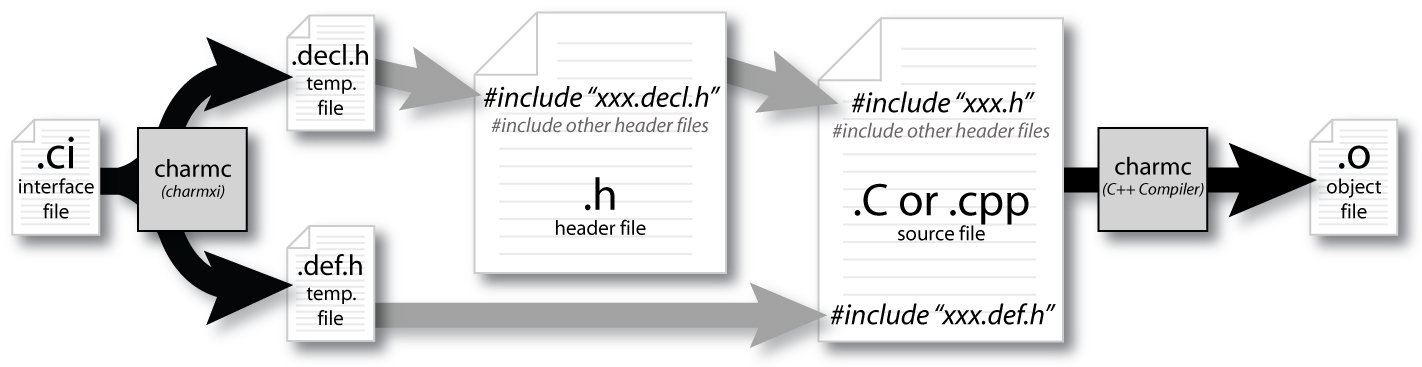
\includegraphics[width=0.9\textwidth]{figures/charmCompile.jpg}
   \end{center}
\end{frame}

\begin{frame}
  \frametitle{Building Charm++}
  \begin{itemize}
  \item git clone http://charm.cs.uiuc.edu/gerrit/charm
  \item ./build $<$TARGET$>$ $<$ARCH$>$ $<$OPTS$>$
  \item TARGET = Charm++, AMPI, bgampi, LIBS etc.
  \item ARCH = net-linux-x86\_64, multicore-darwin-x86\_64, pamilrts-bluegeneq etc.
  \item OPTS = --with-production, --enable-tracing, xlc, smp, -j8 etc.
  \item http://charm.cs.illinois.edu/manuals/html/charm++/A.html
  \end{itemize}
\end{frame}

\begin{frame}
  \frametitle{Hello World Example}
  \begin{itemize}
    \item Compiling
      \begin{itemize}
      \item \texttt{charmc hello.ci}
      \item \texttt{charmc -c hello.C}
      \item \texttt{charmc -o hello hello.o}
      \end{itemize}
    \item Running
      \begin{itemize}
      \item \texttt{./charmrun +p7 ./hello}
      \item The \texttt{+p7} tells the system to use seven cores
      \end{itemize}
    \end{itemize}
\end{frame}

